

\chapter{The surface code}

\begin{figure}[h]
  \centering
  \begin{tikzpicture}
    \DRAWTORIC{3}
    \draw [arrow] (-1,0 |- N-0-2-1) node [align=right, left] {qubit/edge} -- (N-0-2-1);
    \node (plaquette) at ($(N-0-1-0)!0.5!(N-0-0-0)$) {};
    \node (star) at ($(N-1-0-1)!0.5!(N-1-1-1)$) {};
    \draw [arrow] (-1,0 |- plaquette)  node [align=right, left] {face} -- (plaquette);
    \draw [arrow] (-1,0 |- N-1-0-1) node [align=right, left] {vertex} to [out=0, in=225] (star);
    \node [align=left, right] at (3*\s + .5, .5*\s) {periodic boundary};

  \end{tikzpicture}
  \caption{The toric code is defined as a $L\times L$ lattice (here $L=3$) with periodic boundary conditions. The edges on the lattice, which represents the qubits, make up faces and vertices.}\label{sf:fig_toriclattice}
\end{figure}

The variant of the stabilizer codes that we are going to explore in this thesis is Kitaev's \emph{surface code} \cite{kitaev2003fault}, which is of the category of \emph{topological codes}. Among this category, the surface code is preferable as it offers the highest error tolerance under realise noise channels and requires only local stabilizer measurements of physically neighboring qubits. Two variants of the surface code will be considered here, the \emph{toric code} in section \ref{sec:surface_toric} and the \emph{planar code} in section \ref{sec:surface_planar}, and various decoders are detailed in \ref{sec:surface_decoders}.


\section{The toric code}\label{sec:surface_toric}

The \emph{toric code} is defined by arranging qubits on the edges of a square lattice with periodic boundary conditions, as seen in Figure \ref{sf:fig_toriclattice}. The name of the toric code lends itself from the torus, or donut, shape, where any point on the surface of the torus will encounter itself after traversing the torus in either x or y directions. Hence, the top edge of the toric code meets the bottom edge, whereas the left edge meets the right. On a $L\times L$ grid there are $N = 2L^2$ edges and the same amount of physical qubits. This topology of qubit arrangement plays an important part in encoding the logical qubits, which is stored in the non-trivial cycles on the torus. Errors, beneath a certain threshold, will only introduce local effects and does not change these cycles.

\subsection{Stabilizer generators}

To define a stabilizer code, we need to specify the $m$ independent stabilizer generators and the encoded $\bar{X}$ and $\bar{Z}$ operators. On the toric code there are two types of stabilizer generators, \emph{plaquette} and \emph{star} operators, which are associated with the \emph{faces} and \emph{vertices} of the square lattice, respectively.

\begin{figure}
  \centering
  \begin{tikzpicture}
    \DRAWTORIC{3}
    \DRAWPLAQ{1}{1}
    \DRAWERROR{1}{1}{0}{z}
    \DRAWERROR{1}{1}{1}{z}
    \DRAWERROR{1}{0}{0}{z}
    \DRAWERROR{2}{1}{1}{z}
    \node[below of=Bx-1] {(a)};
  \end{tikzpicture}
  \hspace{1cm}
  \begin{tikzpicture}
    \DRAWTORIC{3}
    \DRAWSTAR{1}{1}{3}
    \DRAWERROR{1}{1}{1}{x}
    \DRAWERROR{1}{1}{0}{x}
    \DRAWERROR{1}{2}{1}{x}
    \DRAWERROR{0}{1}{0}{x}
    \node[below of=Bx-1] {(b)};
  \end{tikzpicture}

  \begin{center}
    \hspace{1cm}
    \begin{tikzcd}[row sep={0.5cm,between origins}]
      \lstick{$Q_1$} & \qw & \qw & \qw & \ctrl{5} & \qw \\
      \lstick{$Q_2$}& \qw & \qw & \ctrl{4} & \qw & \qw \\
      \lstick{$Q_3$} & \qw & \ctrl{3} & \qw & \qw & \qw \\
      \lstick{$Q_4$} & \ctrl{2} & \qw & \qw & \qw & \qw \\
      &&&&&&&\\
      \lstick{$P_f$} & \ctrl{} & \ctrl{} & \ctrl{} & \ctrl{} & \meter{}
    \end{tikzcd}
    \begin{tikzcd}[row sep={0.5cm,between origins}]
      \lstick{$Q_1$} & \qw & \qw & \qw & \targ{} & \qw \\
      \lstick{$Q_2$} & \qw & \qw & \targ{} & \qw & \qw \\
      \lstick{$Q_3$} & \qw & \targ{} & \qw & \qw & \qw \\
      \lstick{$Q_4$} & \targ{} & \qw & \qw & \qw & \qw \\
      &&&&&&&\\
      \lstick{$S_v$} & \ctrl{-2} & \ctrl{-3} & \ctrl{-4} & \ctrl{-5} & \meter{}
    \end{tikzcd}
  \end{center}

  \caption{Each face (a) and vertex (b) on the lattice represents a plaquette and star operator, respectively. The non-identity single qubit operators on which they act are indicated. The set of all (but one) plaquettes and vertices make up the stabilizers of the code. }\label{sf:fig_stabilizers}
\end{figure}

\paragraph{Plaquette operators}
For every face $f$ on our lattice, we define a plaquette operator $P_f$, consisting of tensor product of Pauli Z operators on qubits on these edges (see Figure \ref{sf:fig_toriclattice}a),
\begin{equation}\label{eq:sf_plaquette}
  P_f = \bigotimes_{i\in Q(f)} Z_i
\end{equation}
where $Q(f)$ is the set of qubits touching face $f$. On a $L\times L$ grid there are $L^2$ plaquettes.

\paragraph{Star operators}

Similarly, for every vertex $v$ on our lattice, we define a star operator $S_v$, consisting of tensor product of Pauli X operators on qubits neighboring the vertex (see Figure \ref{sf:fig_toriclattice}b),
\begin{equation}\label{eq:sf_star}
  S_v = \bigotimes_{i\in Q(v)} X_i
\end{equation}
where $Q(v)$ is the set of qubits neighboring vertex $v$. On a $L\times L$ grid there are $L^2$ plaquettes.

As each plaquette and star operator needs to be measured, an ancilla qubit is needed at the physical locations of each of these operators. The structure of the full lattice is now clear, as it just a simple square arrangement of alternating data and ancilla qubits in both x and y directions.

The full stabilizer of the code $\m{S}$ can be generated by multiplying elements of the generator operators. Consider two plaquette operators. These two operators will either share one boundary consisting of a qubit, or none. This means that the Pauli Z operator on the boundary qubit will add up to identity as they commute. The result is that the product of the plaquette operators will consists of the overall boundary Pauli operators of the joint plaquette (see Figure \ref{sf:fig_multistab}a).

However, if all plaquettes are applied to the lattice, no boundary will be left. Thus the product of all plaquettes is the identity, which means that the full set of plaquettes are not independent. The full set of plaquette generators can therefore be completed by simply removing a single plaquette from all available plaquettes. There are therefore $L^2 - 1$ independent plaquette operators.

The multiplication of star operators follow the same properties as the plaquette operators described above (see Figure \ref{sf:fig_multistab}b). Thus there are also $L^2 - 1$ independent star operators, which are the star generators. This sums up to $N_S = 2L^2 - 2$ independent stabilizer generators.

\begin{figure}
  \centering
  \begin{tikzpicture}
    \DRAWTORIC{3}
    \DRAWPLAQ{1}{1}
    \DRAWPLAQ{0}{1}
    \DRAWPLAQ{0}{2}
    \DRAWERROR{1}{1}{0}{z}
    \DRAWERROR{1}{0}{0}{z}
    \DRAWERROR{2}{1}{1}{z}
    \DRAWERROR{0}{0}{0}{z}
    \DRAWERROR{0}{1}{1}{z}
    \DRAWERROR{0}{2}{1}{z}
    \DRAWERROR{0}{2}{0}{z}
    \DRAWERROR{1}{2}{1}{z}
    \node[below of=Bx-1] {(a)};
  \end{tikzpicture}
  \hspace{1cm}
  \begin{tikzpicture}
    \DRAWTORIC{3}
    \DRAWSTAR{1}{1}{3}
    \DRAWSTAR{2}{0}{3}
    \DRAWSTAR{2}{1}{3}
    \DRAWERROR{1}{2}{1}{x}
    \DRAWERROR{0}{1}{0}{x}
    \DRAWERROR{2}{2}{1}{x}
    \DRAWERROR{1}{1}{1}{x}
    \DRAWERROR{1}{0}{0}{x}
    \DRAWERROR{2}{0}{1}{x}
    \DRAWERROR{2}{0}{0}{x}
    \DRAWERROR{2}{1}{0}{x}
    \node[below of=Bx-1] {(b)};
  \end{tikzpicture}
  \caption{Multiplication of (a) plaquette and (b) star operators will result in a operator that consists of the Pauli operators that reside on the overall boundary of the joint plaquettes or stars. }\label{sf:fig_multistab}
\end{figure}

\subsection{Dual lattice}
Note that if we shift our lattice half a cell down, and half a cell to the right, we can create a \emph{dual} lattice. This dual lattice has the same size and same boundary conditions as the \emph{primal} lattice, but every plaquette in the primal lattice is a star in the dual lattice, and every star in the primal lattice is a plaquette in the dual lattice. The edges of the dual lattice are plotted with dotted lines in the figures.

This interesting property of \emph{lattice duality} leads to the fact that plaquette and star operators are in fact the same, and we can choose from either that is best suited for the calculation. The multiplication of operators is best pictured in the plaquette picture, for example. For the square lattice in the toric code, the dual lattice is coincidentally also square. For other types of topological codes with non-square lattices, the dual lattice has a different lattice structure than the primal lattice. We will not explore these kind of lattices in this thesis.

\subsection{Encoded qubits}
Since there are $N = L^2$ qubits and $N_S = 2L^2 - 2$ independent stabilizers, we must have $N_L = N - N_S = 2$ encoded qubits and therefore 4 logical operators $\bar{X}_1, \bar{X}_2, \bar{Z}_1$ and $\bar{Z}_2$.

Recall the logical operators consists of the Pauli operators, and must commute with all stabilizer generators, but cannot be part of the stabilizer itself. We can construct the logical operators by starting with, for example, a single Pauli Z operator. It commutes with all plaquette operators trivially. In terms of the star operators, this single Pauli Z operator commutes with all but the two neighboring qubits, as all others apply to different qubits. Adding another Pauli Z operator will shift will of the anticommuting neighboring star operators. We know see that a closed loop of Z operators around the torus does not have neighboring star operators, and therefore commute with all stabilizers. As the torus has two directions we can loop over, these are the logical $\bar{Z}$ operators (see Figure \ref{sf:fig_logical}a-b). Analogously, we can construct the logical $\bar{X}$ operators in the same way (Figure \ref{sf:fig_logical}c-d).

Note that these logical operators are not unique. As the logical operators commute with the stabilizers, these $\bar{X}$ and $\bar{Z}$ operators can be multiplied with e.g. a plaquette or star operator, respectively, which create a diversion from its original path. But as the path still loops around the torus, this is still a valid logical operator.

The logical operators have a minimum length of $L$ qubits, which is also the distance of the toric code. The toric code is therefore a $[L^2,2,L]$ in the [n,k,d] notation. This implies that the toric code might be more robust against errors if the size of the lattice is increased. Later we will see that this is also very much dependent on the type of decoder that is used, and that different decoders will lead to different regimes of error for which this reasoning is true.

\def\QS{10}
\def\s{1}

\begin{figure}
  \centering
  \begin{tikzpicture}
    \DRAWTORIC{5}
    \DRAWERROR{0}{2}{0}{z}
    \DRAWERROR{1}{2}{0}{z}
    \DRAWERROR{2}{2}{0}{z}
    \DRAWERROR{3}{2}{0}{z}
    \DRAWERROR{4}{2}{0}{z}
    \DRAWERROR{3}{0}{1}{z}
    \DRAWERROR{3}{1}{1}{z}
    \DRAWERROR{3}{2}{1}{z}
    \DRAWERROR{3}{3}{1}{z}
    \DRAWERROR{3}{4}{1}{z}
    \begin{pgfonlayer}{edges}
      \draw[synz] (S-0-2) -- (S-5-2);
      \draw[synz] (S-3-4) -- (S-3-5);
    \end{pgfonlayer}
    \node[above=.25cm of S-3-4] {(a)};
    \node[left=.25cm of S-0-2] {(b)};
  \end{tikzpicture}
  \hspace{1cm}
  \begin{tikzpicture}
    \DRAWTORIC{5}
    \DRAWERROR{0}{2}{1}{x}
    \DRAWERROR{1}{2}{1}{x}
    \DRAWERROR{2}{2}{1}{x}
    \DRAWERROR{3}{2}{1}{x}
    \DRAWERROR{4}{2}{1}{x}
    \DRAWERROR{3}{0}{0}{x}
    \DRAWERROR{3}{1}{0}{x}
    \DRAWERROR{3}{2}{0}{x}
    \DRAWERROR{3}{3}{0}{x}
    \DRAWERROR{3}{4}{0}{x}
    \begin{pgfonlayer}{edges}
      \draw[synx] (N-0-2-1) -- (By-2);
      \draw[synx] (Bx-3) -- (N-3-4-0);
    \end{pgfonlayer}
    \node[above=.25cm of N-3-4-0] {(c)};
    \node[right=.25cm of By-2] {(d)};
  \end{tikzpicture}
  \caption{The logical (a) $\bar{X}_1$, (b) $\bar{X}_2$, (c) $\bar{Z}_1$ and (d) $\bar{Z}_2$ operators are the closed loop of $X$ and $Z$ operators, respectively, that go around the two boundaries of the torus. }\label{sf:fig_logical}
\end{figure}

\subsection{Error detection}
As discussed in the previous chapter, errors are detected by measuring the set of stabilizer generators. As we have seen in the previous section, this consists of all but one plaquette operators $P_f$ and all but one star operators $S_v$. Let us first consider to measure all of them.

In the case of a single $Z$ error (Fig \ref{sf:fig_degenerate}a.i), the neighboring plaquette operators will commute with this error, as it consists of Pauli Z operators itself. But the neighboring star operators anticommutes with this error according to equation \ref{qec:eq:stabmeas}. Similarly, a single $X$ error (Fig \ref{sf:fig_degenerate}a.ii) commutes with neighboring star operators but anticommutes with neighboring plaquette operators. A $Y$ error is a combination of $X$ and $Z$ operators and therefore anticommutes with all neighboring generator operators (Fig \ref{sf:fig_degenerate}a.iii).

In the case of two $Z$ errors (Fig \ref{sf:fig_degenerate}a.iv), the star operators between the two errors now commute with the errors, creating a virtual path between them. This is a general property: given any string of errors, the generator operators at the end of the string will anticommute with the errors and measure -1. For $Z$ errors, star operators at the end of strings on the primal lattice will measure -1. The detection of $X$ errors occur in the same way, albeit now the strings of errors is defined on the \emph{dual} lattice, and plaquette errors will measure -1 at the end of these strings.

Since $Z$ and $X$ errors independently affect different types of stabilizer measurements (stars and plaquettes, respectively), these two types of errors can be considered independently in two error correction processes. The two processes are analogous, up to the duality of the lattice. Therefore, for the remainder of the section, only $Z$ errors, which leave a string of errors on the primal lattice, will be considered.

\begin{figure}
  \centering
  \begin{tikzpicture}
    \DRAWTORIC{5}
    \DRAWERROR{1}{2}{0}{z}
    \DRAWERROR{2}{4}{1}{x}
    \DRAWERROR{3}{1}{0}{y}
    \DRAWERROR{1}{0}{0}{z}
    \DRAWERROR{0}{0}{0}{z}
    \DRAWPLAQ{1}{4}
    \DRAWPLAQ{2}{4}
    \DRAWSTAR{1}{2}{5}
    \DRAWSTAR{2}{2}{5}
    \DRAWSTAR{0}{0}{5}
    \DRAWSTAR{2}{0}{5}
    \DRAWPLAQ{3}{1}
    \DRAWPLAQ{3}{2}
    \DRAWSTAR{3}{1}{5}
    \DRAWSTAR{4}{1}{5}
    \begin{pgfonlayer}{edges}
      \draw[synz] (N-0-0-0) -- (N-1-0-0);
    \end{pgfonlayer}
    \node[below=.25cm of Bx-2] {(a)};
    \node[script] at (P-1-2) {\textit{(i)}};
    \node[script] at (P-1-4) {\textit{(ii)}};
    \node[script] at (P-3-1) {\textit{(iii)}};
    \node[script] at (P-1-0) {\textit{(iv)}};

  \end{tikzpicture}
  \hspace{1cm}
  \begin{tikzpicture}
    \DRAWTORIC{5}
    \DRAWERROR{0}{2}{0}{z}
    \DRAWERROR{2}{2}{0}{z}
    \DRAWERROR{3}{2}{0}{z}
    \DRAWERROR{4}{2}{0}{z}
    \DRAWSTAR{1}{2}{5}
    \DRAWSTAR{2}{2}{5}
    \begin{pgfonlayer}{edges}
      \draw[synz] (N-0-2-0) -- (S-0-2) (N-2-2-0) -- (S-5-2);
    \end{pgfonlayer}
    \node[below=.25cm of Bx-2] {(b)};
  \end{tikzpicture}

  \hspace{1cm}
  \begin{tikzpicture}
    \DRAWTORIC{5}
    \DRAWERROR{1}{2}{1}{z}
    \DRAWERROR{1}{1}{1}{z}
    \DRAWERROR{1}{0}{0}{z}
    \DRAWERROR{2}{0}{1}{z}
    \DRAWERROR{2}{4}{1}{z}
    \DRAWERROR{2}{3}{1}{z}
    \DRAWSTAR{1}{2}{5}
    \DRAWSTAR{2}{2}{5}
    \begin{pgfonlayer}{edges}
      \draw[synz] (N-1-2-1) -- (S-1-0) -- (S-2-0) -- (S-2-5) (S-2-4) -- (N-2-3-1);
    \end{pgfonlayer}
    \node[below=.25cm of Bx-2] {(c)};
  \end{tikzpicture}
  \hspace{1cm}
  \begin{tikzpicture}
    \DRAWTORIC{5}
    \DRAWERROR{0}{2}{0}{z}
    \DRAWERROR{4}{2}{0}{z}
    \DRAWERROR{4}{2}{1}{z}
    \DRAWERROR{4}{1}{1}{z}
    \DRAWERROR{3}{0}{0}{z}
    \DRAWERROR{3}{0}{1}{z}
    \DRAWERROR{3}{4}{1}{z}
    \DRAWERROR{3}{3}{1}{z}
    \DRAWERROR{2}{2}{0}{z}
    \DRAWSTAR{1}{2}{5}
    \DRAWSTAR{2}{2}{5}
    \begin{pgfonlayer}{edges}
      \draw[synz] (N-0-2-0) -- (S-0-2) (N-2-2-0) -- (S-3-2) -- (S-3-4);
      \draw[synz] (S-3-5) -- (S-3-0) -- (S-4-0) -- (S-4-2) -- (S-5-2);
    \end{pgfonlayer}
    \node[below=.25cm of Bx-2] {(d)};
  \end{tikzpicture}
  \caption{(a) Stabilizer generators that anticommute with the error will measure -1, which are (i) the neighboring star operators for a Z error, (ii) the neighboring plaquette operators for an X error, and (iii) both star and plaquette operators for a Y error. In the case of a string of errors (iv), only the stabilizer generators at the end of these strings will anticommute with the error. Due to code degeneracy, the single Z error in (a.i) $E$ has the syndrome as (b) $E\bar{Z}_1$, (c) $E\bar{Z}_2$ and (d) $E\bar{Z}_1\bar{Z}_2$. }\label{sf:fig_degenerate}
\end{figure}

\subsection{Error correction}

An error $E$ can be corrected by applying it again to the lattice. The error operator $E$ is however unknown. We must therefore try to identify the correct operator given the measured syndrome. As mentioned in the previous chapter, this relationship between error does not always map one-to-one, which it is not in the surface code. An error $E$ can be multiplied with some operator $L$ that commutes with the stabilizer and they will result in the same syndrome.

If $L$ is in the stabilizer $\m{S}$, the product of the identified correction operator $C=E'$ with the real error operator $E$ will leave the code invariant. The resulting operator $CE=L$ is a stabilizer operator. However, the encoded logical operators also commute with the stabilizer, which means that $E$, $E\bar{Z}_1$, $E\bar{Z}_2$, $E\bar{Z}_1\bar{Z}_2$ will all lead to the same syndrome (Fig \ref{sf:fig_degenerate}a-d). Any identified correction operator $C$ can therefore be categorised into four classes of operators, of which only one includes the correct logical operator. The task of choosing most appropriate correction chain is up to the decoders (section \ref{sec:surface_decoders}).

\subsection{Quasiparticle picture}

The processes of error detection and correction can alternatively be presented in the \emph{quasiparticle picture}, where the anticommuting stabilizer measurements act like excitations on the lattice, which behave like the quasiparticles \emph{anyons}. A single error creates a pair of anyons, and a chain of errors causes movement of the anyon on the lattice. A pair of anyons can also annihilate each other when two error chains merge. The correction of errors can thus be viewed of movement of the correction chains until all anyons are annihilated. The quasiparticle picture removes the distracting underlying lattice from the problem, and decoding becomes simply identifying the right pairing between anyons to minimize the chance of a logical error.

\begin{figure}[h]
  \centering
  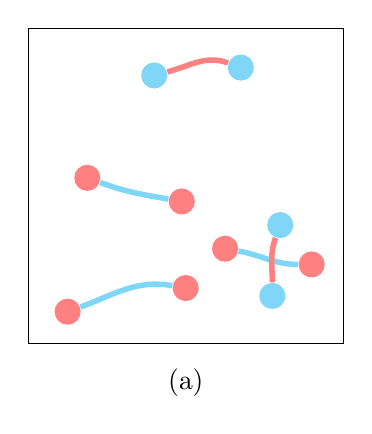
\begin{tikzpicture}
    \draw (0,0) rectangle (4,4);
    \node[circle, fill=red!50, minimum size=4] (N1) at (0.5,0.4) {};
    \node[circle, fill=red!50, minimum size=4] (N2) at (2,0.7) {};
    \node[circle, fill=red!50, minimum size=4] (N3) at (2.5,1.2) {};
    \node[circle, fill=red!50, minimum size=4] (N4) at (3.6,1) {};
    \node[circle, fill=red!50, minimum size=4] (N5) at (0.75,2.1) {};
    \node[circle, fill=red!50, minimum size=4] (N6) at (1.95,1.8) {};
    \node[circle, fill=cyan!50, minimum size=4] (N7) at (1.6, 3.4) {};
    \node[circle, fill=cyan!50, minimum size=4] (N8) at (2.7, 3.5) {};
    \node[circle, fill=cyan!50, minimum size=4] (N9) at (3.2, 1.5) {};
    \node[circle, fill=cyan!50, minimum size=4] (N10) at (3.1, 0.6) {};
    \draw[cyan!50, line width = 2] (N1) to[in=170, out=20] (N2);
    \draw[cyan!50, line width = 2] (N3) to[in=180, out=-10] (N4);
    \draw[cyan!50, line width = 2] (N5) to[in=170, out=-20] (N6);
    \draw[red!50, line width = 2] (N7) to[in=160, out=15] (N8);
    \draw[red!50, line width = 2] (N9) to[in=90, out=250] (N10);
    \node at (2, -.5) {(a)};
  \end{tikzpicture}
  \hspace{1cm}
  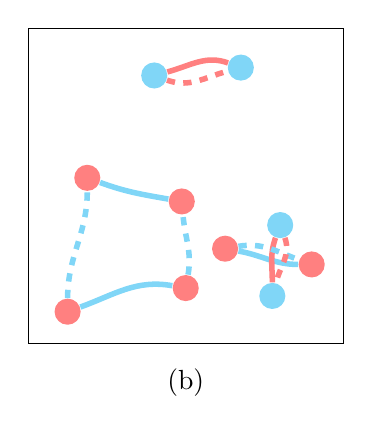
\begin{tikzpicture}
    \draw (0,0) rectangle (4,4);
    \node[circle, fill=red!50, minimum size=4] (N1) at (0.5,0.4) {};
    \node[circle, fill=red!50, minimum size=4] (N2) at (2,0.7) {};
    \node[circle, fill=red!50, minimum size=4] (N3) at (2.5,1.2) {};
    \node[circle, fill=red!50, minimum size=4] (N4) at (3.6,1) {};
    \node[circle, fill=red!50, minimum size=4] (N5) at (0.75,2.1) {};
    \node[circle, fill=red!50, minimum size=4] (N6) at (1.95,1.8) {};
    \node[circle, fill=cyan!50, minimum size=4] (N7) at (1.6, 3.4) {};
    \node[circle, fill=cyan!50, minimum size=4] (N8) at (2.7, 3.5) {};
    \node[circle, fill=cyan!50, minimum size=4] (N9) at (3.2, 1.5) {};
    \node[circle, fill=cyan!50, minimum size=4] (N10) at (3.1, 0.6) {};
    \draw[cyan!50, line width=2] (N1) to[in=170, out=20] (N2);
    \draw[cyan!50, line width=2] (N3) to[in=180, out=-10] (N4);
    \draw[cyan!50, line width=2] (N5) to[in=170, out=-20] (N6);
    \draw[red!50, line width=2] (N7) to[in=160, out=15] (N8);
    \draw[red!50, line width=2] (N9) to[in=90, out=250] (N10);
    \draw[cyan!50, dashed, line width=2] (N1) to[out=90, in=270] (N5);
    \draw[cyan!50, dashed, line width=2] (N2) to[out=80, in=275] (N6);
    \draw[cyan!50, dashed, line width=2] (N3) to[out=10, in=160] (N4);
    \draw[red!50, dashed, line width=2] (N7) to[out=-20, in=195] (N8);
    \draw[red!50, dashed, line width=2] (N9) to[out=290, in=75] (N10);
    \node at (2, -.5) {(b)};
  \end{tikzpicture}
  \hspace{1cm}
  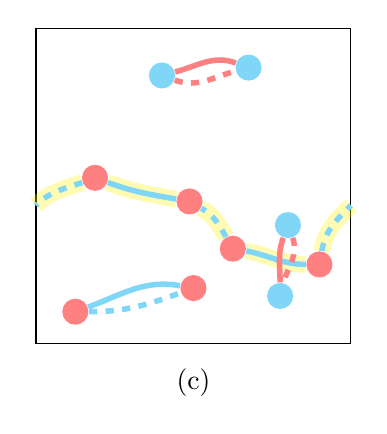
\begin{tikzpicture}
    \draw (0,0) rectangle (4,4);
    \node[circle, fill=red!50, minimum size=4] (N1) at (0.5,0.4) {};
    \node[circle, fill=red!50, minimum size=4] (N2) at (2,0.7) {};
    \node[circle, fill=red!50, minimum size=4] (N3) at (2.5,1.2) {};
    \node[circle, fill=red!50, minimum size=4] (N4) at (3.6,1) {};
    \node[circle, fill=red!50, minimum size=4] (N5) at (0.75,2.1) {};
    \node[circle, fill=red!50, minimum size=4] (N6) at (1.95,1.8) {};
    \node[circle, fill=cyan!50, minimum size=4] (N7) at (1.6, 3.4) {};
    \node[circle, fill=cyan!50, minimum size=4] (N8) at (2.7, 3.5) {};
    \node[circle, fill=cyan!50, minimum size=4] (N9) at (3.2, 1.5) {};
    \node[circle, fill=cyan!50, minimum size=4] (N10) at (3.1, 0.6) {};
    \draw[yellow, line width=6, opacity=.3] (N3) to[in=180, out=-10] (N4);
    \draw[yellow, line width=6, opacity=.3] (N5) to[in=170, out=-20] (N6);
    \draw[yellow, line width=6, opacity=.3] (N3) to[out=120, in=-30] (N6);
    \draw[yellow, line width=6, opacity=.3] (N5) to[out=200, in=45] (0, 1.75);
    \draw[yellow, line width=6, opacity=.3] (N4) to[out=80, in=225] (4, 1.75);
    \draw[cyan!50, line width=2] (N1) to[in=170, out=20] (N2);
    \draw[cyan!50, line width=2] (N3) to[in=180, out=-10] (N4);
    \draw[cyan!50, line width=2] (N5) to[in=170, out=-20] (N6);
    \draw[red!50, line width=2] (N7) to[in=160, out=15] (N8);
    \draw[red!50, line width=2] (N9) to[in=90, out=250] (N10);
    \draw[cyan!50, dashed, line width=2] (N1) to[out=0, in=200] (N2);
    \draw[cyan!50, dashed, line width=2] (N3) to[out=120, in=-30] (N6);
    \draw[cyan!50, dashed, line width=2] (N5) to[out=200, in=45] (0, 1.75);
    \draw[cyan!50, dashed, line width=2] (N4) to[out=80, in=225] (4, 1.75);
    \draw[red!50, dashed, line width=2] (N7) to[out=-20, in=195] (N8);
    \draw[red!50, dashed, line width=2] (N9) to[out=290, in=75] (N10);
    \node at (2, -.5) {(c)};
  \end{tikzpicture}
  \caption{The quasiparticle picture of stabilizer measurements. Anticommuting stabilizers behave as anyons (circles), where a chain of errors (lines) creates a pair of anyons. Figure (b) shows a successful decoding of (a). Figure (c) shows a pairing that resulted in a correction operator that is in a different class as the error operator, which acquires a logical error.}\label{fig:quasiparticle}
\end{figure}

Figure \ref{fig:quasiparticle}a shows the quasiparticle representation of the errors suffered in Figure \ref{sf:fig_degenerate}a, which has suffered Z (blue lines) and X errors (red lines). The corresponding anyons can either be of the star type (red circle) or plaquette type (blue circle). Figure \ref{fig:quasiparticle}b shows a successful decoding. Note that here not all pairs are correctly identified, but the resulting loop still is in the same class of operators. In figure \ref{fig:quasiparticle}c the correction has failed as the resulting loop in the correction is in a difference class compared to the error. As the loop still commutes with the stabilizer, no error can be detected, but the encoded qubit has acquired a logical error.

\subsection{Code threshold}
Since the distance $d$ of the toric code on a $L\times L$ is $L$, we would expect that we can improve the robustness of the code by increasing the lattice size $L$. However, this also increases the total number of errors in the lattice, that adds an increased level of complexity in choosing the correct correction operator.

In practice, there is a trade-off between the positive effect of a larger code distance and the negative effect of larger number of errors. When the error rate $p$ is low, the positive effect outweighs the negative and increasing the lattice $L$ will increase the probability of successful error correction $p_C$. When the error rate is large, the negative effect outweighs the positive and increasing $p$ will decrease $p_C$. The point of transition in the error rate is called the \emph{code threshold} $p_{th}$.

The code threshold is not the only parameter that determines the potential of a certain code for practical use. The behavior for error rates far below the threshold is also important, as is the number of physical qubits needed to achieve the sought after level of error suppression. Nevertheless, the code threshold provides us with a very easy and useful tool to benchmark different codes and different decoding algorithms, and to compare them with each other. Therefore, in this thesis we will heavily rely on the value of the code threshold. The value of the threshold is heavily dependent on the chosen error model and the physical conditions of the stabilizer measurements. To compare different decoding algorithms, we therefore will use independent and identically distributed errors (i.i.d. noise), which is the \emph{independent noise model} from section \ref{qec:sec_errormodels}.

For the toric code, when the only source of errors is i.i.d. noise under the independent noise model, and all measurements can be made perfectly, the \emph{optimal threshold} has been proven to be 10.9\% (see section \ref{sec:optimal_decoder}). However, to achieve this value, one needs to consider all possible error configurations on the lattice to identify the correction operator $C$ that is most likely to be equal to the error operator $E$. This is a computationally heavy task that scales exponentially with the lattice size. It is therefore an impractical approach in reality.

Luckily, there exists other decoding algorithms that can find a solution much faster, albeit at the cost of reducing the code threshold. Edmond's \emph{Minimum Weight Perfect Matching} (MWPM) decoder scales cubic with the system, which allows for faster decoding, and achieves a code threshold of 10.3\% (section \ref{sec:MWPMdecoder}). Including faulty measurements the threshold drops down to 2.9\%. The \emph{Union-Find} decoder is a relatively new addition to the set of decoders for the surface code. It scales \emph{almost} linearly with the system, and has a code threshold of 9.9\% (section \ref{sec:UFdecoder}). In this thesis, we will try to combine certain properties of different decoders. In particular, we have created a heuristic for minimum weight which can be applied to the Union-Find decoder.

\section{The planar code}\label{sec:surface_planar}

Another variant of the surface code is the \emph{planar code}, which disposes the periodic boundary conditions of the torus. This allows the qubits to be placed onto a flat 2D surface. For real systems in which the qubits physically interact with each other, this is a huge benefit. Therefore, in this thesis, we will consider both toric and planar variants of the surface code.



\def\QS{15}
\def\s{1.5}

\begin{figure}[h]
  \centering
  \begin{tikzpicture}
    \DRAWPLANAR{6}
    \DRAWPLAQ{1}{3}
    \DRAWEPLAQ{0}{5}
    \DRAWSTAR{3}{3}{4}
    \DRAWESTAR{2}{5}
    \DRAWERROR{1}{3}{0}{z}
    \DRAWERROR{1}{3}{1}{z}
    \DRAWERROR{1}{2}{0}{z}
    \DRAWERROR{2}{3}{1}{z}
    \DRAWERROR{0}{4}{0}{z}
    \DRAWERROR{0}{5}{0}{z}
    \DRAWERROR{1}{5}{1}{z}
    \DRAWERROR{1}{5}{0}{x}
    \DRAWERROR{2}{5}{0}{x}
    \DRAWERROR{2}{5}{1}{x}
    \DRAWERROR{2}{3}{0}{x}
    \DRAWERROR{3}{3}{0}{x}
    \DRAWERROR{3}{3}{1}{x}
    \DRAWERROR{3}{4}{1}{x}
    \DRAWERROR{4}{0}{0}{x}
    \DRAWERROR{4}{1}{0}{y}
    \DRAWERROR{4}{2}{0}{x}
    \DRAWERROR{4}{3}{0}{x}
    \DRAWERROR{4}{4}{0}{x}
    \DRAWERROR{4}{5}{0}{x}
    \DRAWERROR{0}{1}{0}{z}
    \DRAWERROR{1}{1}{0}{z}
    \DRAWERROR{2}{1}{0}{z}
    \DRAWERROR{3}{1}{0}{z}
    \DRAWERROR{5}{1}{0}{z}
    \begin{pgfonlayer}{edges}
      \draw[synz] (N-0-1-0) -- (N-5-1-0);
      \draw[synx] (N-4-5-0) -- (N-4-0-0);
    \end{pgfonlayer}

    \node[script] at (P-1-3) {(c)};
    \node[script] at (S-3-3) {(d)};
    \node[script] at (P-0-5) {(a)};
    \node[script] at (S-2-5) {(b)};
    \node[above=.25cm of N-4-5-0] {(f)};
    \node[left=.25cm of N-0-1-0] {(e)};
  \end{tikzpicture}


  \caption{The planar code with lattice size $L=4$, which includes $N = 2L^2-2L+1$ qubits and $N_S = 2L^2-2L$ independent stabilizers. The boundary is defined by the (a) EDGE-plaquette and (b) EDGE-star operators, which exist next to the known (c) plaquette and (d) star operators, similar to the toric code. The planar codes encodes 1 logical qubit, which is represented by the logical (e) $\bar{Z}$ and (f) $\bar{X}$ operators.}\label{sf:fig_planar}
\end{figure}

\paragraph{Stabilizer generators}
There are a few key differences between the planar and toric codes. First of all, a new type of stabilizer generators define the non-periodic boundary of the lattice, which are referred to as \emph{EDGE operators}. These EDGE operators have only 3 neighboring qubits and are therefore the tensor product of 3 Pauli operators. The EDGE-plaquette operators lie at the east and west boundaries of the lattice (Figure \ref{sf:fig_planar}a) and the EDGE-star $S_{vE}$ operators lie at the north and south boundaries of the lattice (Figure \ref{sf:fig_planar}b). In the middle of the lattice, the bulk of the stabilizer generators still consist of 4 Pauli operators, identical to the ones in the toric code (Figure \ref{sf:fig_planar}c-d). Note that the stabilizer generators are still defined by equation \ref{eq:sf_plaquette} and \ref{eq:sf_star}, but now the relevant faces and vertices contain three neighboring qubits.

\paragraph{Stabilizer violoations}
A second key difference is that now not all errors will cause two stabilizer violations. In the bulk of the qubits on the lattice, a single error will still cause two neighboring stabilizers to measure -1, or create two anyons. At the boundary however, it now may be the case that an error is only included in one plaquette or star operator. This will also mean the decoding in the quasiparticle picture requires a slightly different approach.

\paragraph{Logical qubits}
Furthermore, we can inspect that a planar surface of dimension $L$ has $N = 2L^2-2L+1$ physical qubits. We can also find that there are $2L^2-2L$ stabilizer generators. As the boundary is now non-periodic, all generators are now independent, and therefore the number independent generators is $N_S = 2L^2-2L$. This means that the planar code encodes $N_L = N-N_S = 1$ a single logical qubit. The logical $\bar{X}$ and $\bar{Z}$ operators are pictured in Figure \ref{sf:fig_planar}e-f.\\

Other properties of the planar code are very similar to the toric code. The \emph{dual lattice} also exists for the planar code, for example. But the dual lattice exists at a 90 angle compared to the primary lattice. Also, as the bulk of the lattice still consists of 4-Pauli operator stabilizers, the decoding algorithms for the planar code is very similar to the toric code. It is due to the boundary that some slight alterations are needed, as we will see in the next section.

\section{Decoders}\label{sec:surface_decoders}
\subsection{The optimal decoder}\label{sec:optimal_decoder}
\subsection{Minimum Weight Perfect Matching}\label{sec:MWPMdecoder}
\subsection{The Union-Find decoder}\label{sec:UFdecoder}

Even the fastest MWPM algorithms still have a quadratic time complexity of $\m{O}(n^2\sqrt{n})$, where $n$ is the number of qubits. In order to realistically utilize a decoder with increasing decoding success rates using increasing lattice size, we would need to have a better time complexity. Luckily, an alternative algorithm called the Peeling Decoder has been developed which can solve errors over the erasure channel with a linear time complexity $\m{O}(n)$ \cite{delfosse2017linear}. The Union-Find Decoder builds on top of the Peeling Decoder to solve for Pauli errors with a time complexity of $\m{O}(n\alpha(n))$, where $\alpha$ is an inverse Ackermann function, which is smaller than 3 for any practical input size \cite{delfosse2017almost}. However, these algorithms have a tradeoff in the form of a decrease in the error threshold, and has the reported value of $p_{UF} = 9.2\%$.

A topic of interest will be weighted growth function for the Union-find decoder. This function of the algorithm will increase the error threshold to $p_{UF} = 9.9\%$, but has not been fully described in its publication.  In this section, we will describe the original Peeling decoder and the Union-Find decoder.   \\

\subsubsection{The Peeling decoder}
Let $\varepsilon \subset E$ be an erasure, a set of qubits on which an erasure error occurs, and let $\sigma \subset S$ be the measured error syndrome, the subset of stabilizer generators which anticommute with the erasure errors. In the absence of Pauli errors, all errors $P$ must lie inside the erasure. Therefore, for any pair of stabilizer generators in $\sigma$, the path of errors must also be in the erasure, which can be denoted by $P\subset \varepsilon$. Furthermore, due to the fact that errors $P$ are randomly distributed, any coset of errors and stabilizers $P\cdot S$ that solves the error syndrome $\sigma$ is the most likely coset. These features of an erasures forms the basis of the Peeling decoder. In order to find a coset of $P \cdot S$, the decoder reduces the size of the erasure by peeling edges from the erasure, while keeping the syndromes at the new boundary of the erasure. Elements of the syndrome can be moved by applying an correction on the adjacent qubit. At the end, the entire erasure is peeled or removed, and all corrections will have removed the errors up to a stabilizer.

\tikzset{
  anyon/.style={circle, fill=OrangeRed, minimum size=.2cm, inner sep=0},
  erasure/.style={NavyBlue, very thick},
  correction/.style={Green, very thick},
  description/.style={align=#1, anchor=west, text width=4cm},
  description/.default={left},
  error/.style={text=black, pos=0.5}
  }
\tikzset{
  anyon/.style={circle, fill=OrangeRed, minimum size=.2cm, inner sep=0},
  erasure/.style={NavyBlue, very thick},
  correction/.style={Green, very thick},
  description/.style={align=#1, text width=4cm},
  description/.default={left},
  error/.style={text=black, pos=0.5}
  }

\begin{figure}
  \centering
  \begin{tikzpicture}[on grid, scale=0.8]
    \node at (0,4) {a)};
    \draw[step=1cm,gray,thin] (0.1,0.1) grid (3.9,3.9);
    \draw[erasure] (1,1) -- (2,1) node[error]{$X$} -- (3,1) -- (3,2) -- (2,2) -- (1,2) -- cycle node[error]{$X$};
    \draw[erasure] (1,2) -- (1,3) -- (2,3) node[error]{$X$} -- (2,2);
    \node[description={center}] at (2, -.5) {initial state};

    \begin{scope}[shift={(6,0)}]
      \node at (0,4) {b)};
      \draw[step=1cm,gray,thin] (0.1,0.1) grid (3.9,3.9);
      \draw[erasure] (1,1) -- (2,1) node[anyon]{} -- (3,1) -- (3,2) -- (2,2) -- (1,2) node[anyon] (a) {} -- cycle;
      \draw[erasure] (a) -- (1,3) node[anyon]{} -- (2,3) node[anyon]{}-- (2,2);
      \node[description={center}] at (2, -.5) {identify syndrome};
    \end{scope}

    \begin{scope}[shift={(12,-.5)}]
      \draw[thin] (0,4) -- ++(.5,0) ++(.5,0) node[anchor=west]{normal edge};
      \draw[thin] (0,3) -- ++(.5,0) node[error]{$X$} ++(.5,0) node[anchor=west]{Pauli error};
      \draw[erasure] (0,2) -- ++(.5,0) ++(.5,0) node[anchor=west, text=black]{erased edge};
      \draw[thin] (0,1) -- ++(.5,0) node[anyon,pos=.5]{} ++(.5,0) node[anchor=west]{syndrome};
      \draw[correction] (0,0)   -- ++(.5,0) ++(.5,0) node[anchor=west,text=black]{correction edge};
    \end{scope}

    \begin{scope}[shift={(0,-6)}]
      \node at (0,4) {c)};
      \draw[step=1cm,gray,thin] (0.1,0.1) grid (3.9,3.9);
      \draw[erasure] (1,3) node[anyon]{} -- (2,3) node[anyon]{} -- (2,2) -- (1,2) node[anyon]{} -- (1,1) -- (2,1) node[anyon]{} -- (3,1) -- (3,2);
      \node[description={center}] at (2, -.5) {construct $F_{\varepsilon}$};
    \end{scope}

    \begin{scope}[shift={(6,-6)}]
      \node at (0,4) {d)};
      \draw[step=1cm,gray,thin] (0.1,0.1) grid (3.9,3.9);
      \draw[erasure] (1,3) node[anyon]{} -- (2,3) node[anyon]{} -- (2,2) -- (1,2) node[anyon]{} -- (1,1) -- (2,1) node[anyon](a){};
      \draw[erasure, dashed] (a) -- (3,1) node[pos=0, below, text=black]{$v$} node[pos=0.5, above]{$e$} node[pos=1, below, text=black]{$u$};
      \node[description={center}] at (2, -.5) {peel $e=(u,v), u \notin \sigma$};
    \end{scope}

    \begin{scope}[shift={(12,-6)}]
      \node at (0,4) {e)};
      \draw[step=1cm,gray,thin] (0.1,0.1) grid (3.9,3.9);
      \draw[erasure] (1,3) node[anyon]{} -- (2,3) node[anyon]{} -- (2,2) -- (1,2) node[anyon]{} -- (1,1);
      \draw[erasure, dashed] (1,1) node[below, text=black]{$v$} -- (2,1) node[anyon]{} node[pos=0.5, above]{$e$} node[below, text=black]{$u$};
      \node[description={center}] at (2, -.5) {peel $e=(u,v), u \in \sigma$};
    \end{scope}

    \begin{scope}[shift={(0,-12)}]
      \node at (0,4) {f)};
      \draw[step=1cm,gray,thin] (0.1,0.1) grid (3.9,3.9);
      \draw[erasure] (1,3) node[anyon]{} -- (2,3) node[anyon]{} --  (2,2) -- (1,2) node[anyon]{} -- (1,1) node[anyon](a){};
      \draw[correction] (a) node[below, text=black]{$v$} -- (2,1) node[pos=0.5, above]{$e$} node[below, text=black]{$u$};
      \node[description={center}] at (2, -.5) {flip $u,v$, add $e$ to $C$};
    \end{scope}

    \begin{scope}[shift={(6,-12)}]
      \node at (0,4) {g)};
      \draw[step=1cm,gray,thin] (0.1,0.1) grid (3.9,3.9);
      \draw[correction] (1,3) -- (2,3) node[error]{$X$} (2,1) -- (1,1) node[error]{$X$} -- (1,2) node[error]{$X$};
      \node[description={center}] at (2, -.5) {apply correction set $C$};
    \end{scope}

    \begin{scope}[shift={(12,-12)}]
      \node at (0,4) {h)};
      \draw[step=1cm,gray,thin] (0.1,0.1) grid (3.9,3.9);
      \node[description={center}] at (2, -.5) {end state};
    \end{scope}
  \end{tikzpicture}
  \caption{Schematic representation of the Peeling decoder. On an erasure $\m{E}\subset E$ (a), there may be some Pauli errors $P\subset \m{E}$ that anticommutes with some stabilizer measurements (b) that is identified as the syndrome $\sigma$. The first step is to construct a spanning forest $F_\m{E}\subset \m{E}$, a fully connected acyclic graph. Next the decoder sequentially removes leaf edges $e=(u,v)$ from the forest that connect to the forest via only one vertex $v$. If $u\in\sigma$ (e), remove $u$ from $\sigma$, flip $v$ in $\sigma$ and the edge $e$ is added to the correction set $C$ (f). If $u \notin \sigma$, move on the the next leaf. After applying the correction set $C$, all errors on the lattice commutes with the stabilizers, potentially solving the error (h).}
\end{figure}

\todo[inline]{use capitals for sets $\Sigma$, and lowercase $\sigma$ for elements in the set}

We will now describe the Peeling decoder as is presented in Algorithm \ref{algo:peel}. In step 1, we will remove all cycles present in $\varepsilon$. We construct a spanning forest $F_\varepsilon$ inside erasure $\varepsilon$, the maximal subsect of edges of $\varepsilon$ that contains no cycles and spans all vertices of $\varepsilon$. From here, we loop over all edges in $F_\varepsilon$ (step 3), starting at a leaf edge $e = \{u,v\}$, removing the leaf edge from $F_\varepsilon$ (step 4), and conditionally add the edge to the correction set $\kappa$ if the pendant vertex $u$ is in $\sigma$ (step 6). If the correction is applied immediately, we can see that the pendant vertex $u$ is removed from $\sigma$ and that the value of $v$ is flipped in $\sigma$. Edges on a branch in the forest will be added to $\kappa$ until $v \in \sigma$, or a generator will be continuously moved from $u$ to $v$ until it encounters another generator, creating a correction path between two syndrome pairs.

\begin{lemma}\label{lem:forestofgraph}
  A forest $F$ is an undirected graph in which any two vertices are connected by at most one path. A forest $F_G$ of some graph $G$ is one in which some edges is removed such that there are no cycles in the graph, which satisfies the forest requirement.
\end{lemma}

\begin{algo}[algotitle=Peeling decoder \cite{delfosse2017linear}, label=algo:peel]
  \begin{algorithm}[H]
    \KwData{A graph $G = (V,E)$, an erasure $\varepsilon \subset E$ and syndrome $\sigma \subset V$}
    \KwResult{Correction set $\kappa \subset E$}
    \BlankLine
    construct a spanning forest $F_\varepsilon$ of $\varepsilon$\;
    initialize $\kappa$ by $\kappa = {\emptyset}$\;
    \While{$F_\varepsilon \neq \emptyset$}{
    pick a leaf edge $e = {u,v}$ with pendant vertex $u$, remove $e$ from $F_\varepsilon$ \;
    \If{$u \in \sigma$}{
      add $e$ to $\kappa$, remove $u$ from $\sigma$ and flip $v$ in $\sigma$}
    \Else{do nothing}
    }
    \KwRet{$\kappa$}
  \end{algorithm}
\end{algo}

\noindent Note that due the flipping of both $u$ and $v$ in $\sigma$, the parity of the number of generators in $\sigma$ is always preserved. The peeling decoder can therefore always solve erasures with an even parity, as the size of $\sigma$ will drop until at the end the syndrome will be empty $\sigma = \emptyset$, and call errors are corrected up to a stabilizer. This is always the case in the absence of measurement and Pauli errors, as all errors within the erasure either add or remove an even number of generators to or from $\sigma$.

\paragraph{Time complexity of the Peeling decoder}
The spanning forest $F_\varepsilon$ can be constructed in linear time. Also, the loop over the forest can be operated in linear if the list of leaves is pre-computed and updated during the loop. Thus the Peeling decoder has a linear time complexity in the size of the erasure $\m{O}(\abs{\varepsilon})$ and therefore also in the number of qubits $\m{O}(n)$.

\subsubsection{Growing erasures}

Now in the presence of Pauli errors, errors can occur on edges that are now not part of the erasure, and odd parity clusters can occur. Clusters that consists from only a single generator also exist, which are just end-points of syndromes caused by Pauli errors. We must therefore make an erasure $\varepsilon$ from the syndrome $\sigma$ that is compatible with the peeling decoder, which contains only even parity clusters. To do this, we can attractively grow the clusters with an odd parity by an half-edge on the boundaries on the clusters. When two odd parity clusters meet, the merged cluster will have a even parity, and can now be solved by the peeling decoder.

\paragraph{Union-Find algorithm}

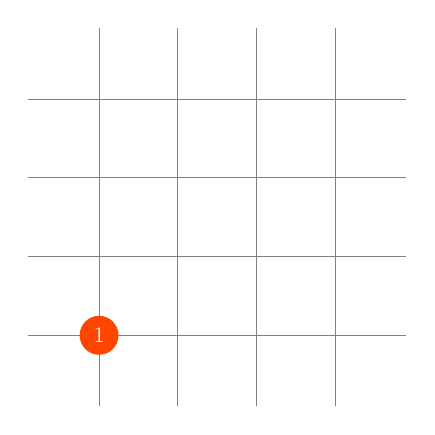
\begin{tikzpicture}
  \draw[step=1cm,gray,thin] (0.1,0.1) grid (4.9, 4.9);
  \node[fill=OrangeRed, circle, text=white, scale=0.8] (N0) at (1, 1) {1};

\end{tikzpicture}

\todo[inline]{add definition of vertex set}
To keep track of the vertices of a cluster, it will be represented as a \emph{cluster tree}, where an arbitrary vertex of the cluster will be the root, and any other vertex will be a child of the root. Whenever an edge $(u,v)$ is fully grown, we will need to traverse the trees of the two vertices $u$ and $v$, and check whether they have the same root; whether they belong to the same cluster. If not, a merge is initiated by making the root of smaller cluster a child of the bigger cluster. These functions, \codefunc{find} and \codefunc{union} respectively, are part of the Union-Find algorithm (not to be confused with the Union-Find decoder) \cite{tarjan1975efficiency}.

\begin{tikzpicture}
  \draw (2,2) circle (0.2);
  \draw (2,2) -- (0,0);)
\end{tikzpicture}

\todo[inline]{syndrome identification, syndrome validation, peeling decoder}

Within the Union-Find algorithm, two features ensure that the complexity of the algorithm is not quadratic. 1). With \textbf{path compression}, as we traverse a tree from child to parent until we reach the root, we make sure that each vertex encountered that we have encountered along the way is pointed directly to the root. This doubles the cost of the \codefunc{find}, but speeds up any future call to any vertex on the traversed path. 2). With \textbf{weighted union}, we make sure to always make the smaller tree a child of the bigger tree. This ensures that the overall length of the path to the root stays minimal. In order to make this happen, we just need to store the size of the tree at the root.

\paragraph{Data structure}
Now it is clear what information is exactly needed to grow the clusters using the Union-Find algorithm. We will need to store the cluster in a sort of cluster-tree. At the root of each tree we store the size and parity of that cluster in order to facilitate weighted union and to select the odd clusters. We will need to store the state of each edge (empty, half-grown, or fully grown) in a table called \codeword{support}. And we need to keep track of the boundary of each cluster in a \codeword{boundary} list.

\paragraph{The routine}
The full routine of the Union-Find decoder as originally described (\cite{delfosse2017almost}, Algorithm 2) is listed in Algorithm \ref{algo:uf}. In line 1-2, we initialize the data structures, and a list of odd cluster roots $\m{L}$. We will loop over this list until it is empty, or that there are no more odd clusters left.

In each growth iteration, we will need to keep track of which clusters have merged onto one, therefore the fusion list $\m{F}$ is initialized in line 4. We loop over all the edges from the \codeword{boundary} of the clusters from $\m{L}$ in line 5, and grow each edge by an half-edge in \codeword{support}. If an edge is fully grown, it is added to $\m{F}$.

For each edge $(u,v)$ in $\m{F}$, we need to check whether the neighboring vertices belong to different clusters, and merge these clusters if they do. This is done using the Union-Find algorithm in line 6. We call \codefunc{find(u)} and \codefunc{find(v)} to find the cluster roots of the vertices. If they do not have the same root, we make one cluster the child of another by \codefunc{union(u,v)}. Note that this does not only merge two existing clusters, also new vertices, which have themselves as their roots, are added to the cluster this way. We also need to combine the boundary lists of the two clusters.

Finally, we need to update the elements in the cluster list $\m{L}$. First, we replace each element $u$ with its potential new cluster root \codefunc{find(u)} in line 7. We can avoid creating duplicate elements by maintaining an extra look-up table that keeps track of the elements $\m{L}$ at the beginning of each round of growth. In line 8, we update the \codeword{boundary} lists of all the clusters in $\m{L}$, and in line 9, even clusters are removed from the list, preparing it for the next round of growth.

\begin{algo}[algotitle=Union-Find decoder \cite{delfosse2017almost}, label=algo:uf]
  \begin{algorithm}[H]
    \KwData{A graph $G = (V,E)$, an erasure $\varepsilon \subset E$ and syndrome $\sigma \subset V$}
    \KwResult{A grown erasure $\varepsilon'$ such that each cluster $\gamma \subset \varepsilon$ is even}
    \BlankLine
    initialize cluster-trees, support and boundary lists for all clusters \;
    initialize list of odd cluster roots $\m{L}$\;
    \While{$\m{L} \neq \emptyset$}{
    initialize fusion list $\m{F}$ \;
    for all $u \in \m{L}$, grow all edges in the boundary list of cluster $C_u$ by a half-edge in support. If the edge is fully grow, add to fusion list $\m{F}$ \;
    for all $e={u,v} \in \m{F}$, if \emph{find($u$)} $\neq$ \emph{find($v$)}, then apply \emph{union($u,v$)}, append boundary list\;
    for all $u \in \m{L}$, replace $u$ with \emph{find($u$)} without creating duplicate elements\;
    for all $u \in \m{L}$, update the boundary list\;
    remove even clusters from $\m{L}$\;
    }
    run peeling decoder with grown erasure $\varepsilon'$
  \end{algorithm}
\end{algo}

\subsubsection{Time complexity of the Union-Find decoder}
